\documentclass[12pt,fleqn]{article}
\usepackage{a4}
\usepackage{graphicx}
\usepackage{psfrag}
\usepackage{amsmath}                     % \boldsymbol{#1}
\usepackage{amssymb}
\usepackage{hangcaption}
\usepackage{Styles/pstricks}
\usepackage{Styles/pst-node}
\usepackage{Styles/fancyheadings}
\usepackage{tocloft}
%-----Tex width---------------------------------
\textwidth 16cm

%-----Line spacing-------------------------------
\renewcommand{\baselinestretch}{1.5}     % 1,1-zeilig

%---------Add dots in TOC-----------------------
\renewcommand{\cftsecleader}{\cftdotfill{\cftdotsep}}

%------Paragraph indention-------------------------------
\setlength{\parskip}{1.5ex plus0.5ex minus0.5ex}

%-----Prevent indent----------------------
\setlength{\parindent}{0em}

%-----Richtiger Abstand fur Einheiten-------------
\def\Unit{\hspace{0.25em}}

%-----Definition of the header--------------------
\pagestyle{fancyplain}
\renewcommand{\sectionmark}[1]{\markboth{Chapter~\thesection.~#1}{#1}}
\renewcommand{\subsectionmark}[1]{\markright{\thesubsection\ #1}}
\rhead[\fancyplain{}{\leftmark}]%
{\fancyplain{\thepage}{\thepage}} \cfoot{} \plainheadrulewidth
0.4pt
%% Otherwise: Overfull \vbox-Warning against fancyheadings-pacakage
%%  idea of: nic@minster.york.ac.uk (Nick Cropper)
\makeatletter
\ifcase \@ptsize \relax % 10pt
  \addtolength{\headheight}{1\p@}
\or % 11pt
  \addtolength{\headheight}{2\p@}
\or % 12pt
  \addtolength{\headheight}{3\p@}
\fi \makeatother

%-----Equations / Figures / Tables numbering according to \ sections
\makeatletter
\renewcommand\theequation{\thesection.\arabic{equation}}
\renewcommand\thefigure{\thesection.\arabic{figure}}
\renewcommand\thetable{\thesection.\arabic{table}}
\@addtoreset{equation}{section} \@addtoreset{figure}{section}
\@addtoreset{table}{section} \makeatother

%-----Useful abbreviations----------------------
\newcommand{\mr}{\mathrm}
\newcommand{\bs}[1]{\mbox{$\boldsymbol{#1}$}}
\newcommand{\degree}[1]{\mbox{$#1^\circ$}}

%\renewcommand{\figurename}{Bild}

%------Bibliography style-----------------------
\bibliographystyle{IEEEtran}

%-----Aufzaehlunstiefe im Literaturverzeichnis---------------
\setcounter{tocdepth}{3}

\begin{document}
\pagenumbering{Roman}
\begin{titlepage}
  \begin{center}
      \vspace*{-4.0cm}
    \begin{figure}[!h]
\centering

\includegraphics[width=0.3\linewidth]{Figures/JKUAT_logo}
%\caption{}
\label{fig:jomologo}
\end{figure}
   \large{Jomo Kenyatta University of Agriculture and Technology}\\
    \large{College of Engineering and Technology}\\
    \large{School of Mechanical, Materials, and Manufacturing Engineering}\\
   \large{Department of Mechatronic Engineering}\\

    ------------------------------------------------------------------------------------------------\\[1.0cm]
    \LARGE{\textbf{Designing a wall-climbing robot\ldots\ldots}}\\[0.6cm]
    \LARGE{\textbf{Final year project (FYP 13-11)
            }}\\[1.5cm]
    %\large{by}\\[0.6cm

    \vspace{0.5cm}
    \large{\textbf{Theodore Kamau (EN292-2025/2012)
            }}\\
     \large{\textbf{Lisa Kimondo~(EN292-2020/2012)
            }}\\[1.0cm]
%     \large{\textbf{Supervisors}}\\
%    \large{Dr.-Ing.~Jackson G. Njiri}\\
%    \large{Prof. George N. Nyakoe}\\
%    \large{\ldots}    \\[0.2cm]\vfill
    \large{\small{\today}}\\
    ------------------------------------------------------------------------------------------------\\[1.5cm]
  \end{center}
\end{titlepage}
%
%\pagenumbering{gobble}% Remove page numbers (and reset to 1)

\addcontentsline{toc}{section}{Declaration}
\section*{Declaration}


We hereby declare that the work contained in this report is original; researched and documented by the undersigned students. It has not been used or presented elsewhere in any form for award of any academic qualification or otherwise. Any material obtained from other parties have been duly acknowledged. We have ensured that no violation of copyright or intellectual property rights have been committed.
\begin{enumerate}
	\item Theodore Kamau\vspace*{.2cm}\\
	Signature\ldots\ldots\ldots\ldots\ldots\ldots\ldots\ldots\ldots\ldots Date\ldots\ldots\ldots\ldots\ldots\ldots\ldots\ldots\ldots\ldots
	\item Lisa Kimondo\vspace*{.2cm}\\
	Signature\ldots\ldots\ldots\ldots\ldots\ldots\ldots\ldots\ldots\ldots Date\ldots\ldots\ldots\ldots\ldots\ldots\ldots\ldots\ldots\ldots
\end{enumerate}

\vspace*{.5cm}
Approved by supervisors:
\begin{enumerate}
	\item Dr.-Ing. Jackson G. Njiri\vspace*{.2cm}\\
	Signature\ldots\ldots\ldots\ldots\ldots\ldots\ldots\ldots\ldots\ldots Date\ldots\ldots\ldots\ldots\ldots\ldots\ldots\ldots\ldots\ldots
	\item Prof. George N. Nyakoe\vspace*{.2cm}\\
	Signature\ldots\ldots\ldots\ldots\ldots\ldots\ldots\ldots\ldots\ldots Date\ldots\ldots\ldots\ldots\ldots\ldots\ldots\ldots\ldots\ldots
	\item Ms. Lucy W. Kariuki\vspace*{.2cm}\\
	Signature\ldots\ldots\ldots\ldots\ldots\ldots\ldots\ldots\ldots\ldots Date\ldots\ldots\ldots\ldots\ldots\ldots\ldots\ldots\ldots\ldots
\end{enumerate}



\clearpage
\tableofcontents
\clearpage
\addcontentsline{toc}{section}{Table of Contents}
\addcontentsline{toc}{section}{List of Figures}
{%
\let\oldnumberline\numberline%
\renewcommand{\numberline}{\figurename~\oldnumberline}%
\listoffigures
\clearpage
\addcontentsline{toc}{section}{List of Tables}
\listoftables
\newpage
\clearpage
\addcontentsline{toc}{section}{List of Abbreviations}
\clearpage
\newpage

\newpage
\addcontentsline{toc}{section}{Abstract}
\section*{Abstract}
\label{sec:}
This project \ldots\ldots




\clearpage
\pagenumbering{arabic}
  \section{Introduction}
\label{sec:introduction}
\subsection{Background}
(Insert your content)

gghjbbnmmm

\subsection{Problem statement}
(Insert your content)
\subsection{Objectives}
(Insert your content)
\subsection{Justification of the study}
(Insert your content)
  \clearpage
  \section{Literature Review}
\label{sec:review}
%
Itemization
\begin{itemize}
\item Item 1.
\item Item 2.
\item \ldots

\end{itemize}

\begin{equation}
\dot{x}=Ax+Bu+B_dw
\end{equation}
%
 Refering a chapter in the main text. For instance Chapter~\ref{sec:review} 
%
\begin{eqnarray} \nonumber
E = 210000\Unit{\mathrm{\frac{N}{mm^2}}}
\end{eqnarray}
%

%
\begin{eqnarray}\nonumber
\rho = 7{,}85\Unit{\mathrm{\frac{g}{cm^3}}}=
7850\Unit{\mathrm{\frac{kg}{m^3}}}.
\end{eqnarray}
%

\begin{equation}
  \Delta \boldsymbol{r}_k= \boldsymbol{r}_{\mathrm{GBE}_k} -
  \boldsymbol{r}_{\mathrm{C}_k} = (x_{\mathrm{GBE}_k} - x_{\mathrm{C}_k},
  y_{\mathrm{GBE}_k} - y_{\mathrm{C}_k})^T = (\Delta x_k,\Delta
  y_k)^T
\end{equation}
%
 $k=2 \dots n$

%
\begin{equation}
  || \boldsymbol{r}_{\mathrm{GBE}_k} -
  \boldsymbol{r}_{\mathrm{C}_k} || \leq  r_{kj},
\end{equation}
%
 $k$  $j$ 
%

\begin{equation}\label{26}
    {\rm rank} \; \boldsymbol{Q}_{\rm B} = {\rm rank} \left[
    \begin{array}{c}
    \bs C \\
    \bs{CA} \\
    \bs{CA}^2 \\
    \vdots \\
    \bs{CA}^{n-1}
    \end{array} \right] = n.
\end{equation}
%

%
\begin{eqnarray}
K_\varphi & = & 3.64\;\mr{\frac{V}{rad}}\quad\mbox{and}\\
K_x & = & 28.32 \;\mr{\frac{V}{m}}.
\end{eqnarray}
%
%
\subsection{Name of a subsection}
\label{subsec:xxxxx}
%
 $q_1,q_2$ and
$q_3$ (see Fig.~\ref{fig:drei_arm}).
%
\subsection{Another subsection}


%\begin{figure}[!htb]
%  \begin{center}
%    \leavevmode
%    \psfrag{F_Last}[][]{\footnotesize{$F_\mathrm{Last}$}}
%    \psfrag{1}[][]{\footnotesize{P$_1$}}
%    \psfrag{2}[r][]{\footnotesize{Lisa$_2$}}
%    \psfrag{3}[][]{\footnotesize{P$_3$}}
%    \psfrag{4}[][]{\footnotesize{P$_4$}}
%    \psfrag{l,m}[][]{\footnotesize{$l, m$}}
%    \psfrag{q1}[][]{\footnotesize{$q_1$}}
%    \psfrag{-q2}[r][]{\footnotesize{$-q_2$}}
%    \psfrag{-q3}[][]{\footnotesize{$-q_3$}}
%    \psfrag{x0}[][]{\footnotesize{$x_0$}}
%    \psfrag{y0}[][]{\footnotesize{$y_0$}}
%    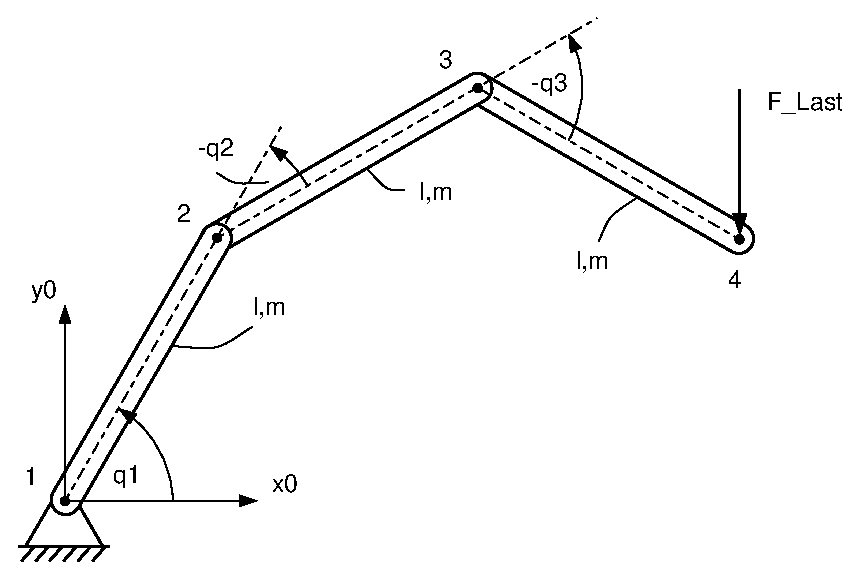
\includegraphics[width=0.64\textwidth]{Figures/drei_arm.eps}
%  \end{center}
%   \hangcaption[The caption for the figure (Add more)]{The caption for the figure should always be at the bottom of the figure\\ The caption can overflow to the next line\ldots}
%  \label{fig:drei_arm}
%\end{figure}



%
\begin{table}[!t]
  \begin{center}
    \leavevmode
    \hangcaption[To appear in the list of tables]{Caption for the table should be at the top of the table\\It can also overflow to next line}   
     \begin{tabular}{rlc}\hline
      First column & Second column & Third column \\ \hline
      1 & 2 & 4\\
      4 & 6 & 23\\
      34 & 2 & 0 \\ \hline
    \end{tabular}
    \label{tab:zweiarmsystemtab}
  \end{center}
\end{table}
%

  \clearpage
    \section{Methodology\ldots}
This is 
  \clearpage
    \section{Expected Outcomes}

%  \clearpage
%  \section{Appendices}
  \clearpage
%----  Bibliography  ----------------------------------------
\markright{References}                               % Erzeugt Kopfzeile
\addcontentsline{toc}{section}{References}            % Literaturverzeichnis ins Inhaltsverzeichnis
\bibliographystyle{Bib/IEEEtran}
\bibliography{Bib/References}                         % BIBTeX
\nocite{Lun01} 

                                     % Falls etwas in die Literaturliste soll, was nicht Referenziert wird
\end{document}
